\documentclass[a4paper,12pt,twoside]{report}
\usepackage{scrextend}
\usepackage[utf8]{vietnam}
\usepackage[top=2cm, bottom=2cm, left=3.5cm, right=2.5cm]{geometry}

\usepackage{graphicx}
\usepackage{indentfirst}
\usepackage{amsmath,amssymb,amsthm}
\usepackage{times}
\usepackage{fix-cm}
\usepackage{type1cm}
\usepackage{subfiles}

% Thiết lập kích thước font 13pt (tương tự báo cáo gốc)
\renewcommand{\normalsize}{\fontsize{13}{15.6}\selectfont}
\renewcommand{\small}{\fontsize{11}{13.2}\selectfont}
\renewcommand{\footnotesize}{\fontsize{10}{12}\selectfont}
\renewcommand{\scriptsize}{\fontsize{8}{9.6}\selectfont}
\renewcommand{\tiny}{\fontsize{6}{7.2}\selectfont}
\renewcommand{\large}{\fontsize{14}{16.8}\selectfont}
\renewcommand{\Large}{\fontsize{16}{19.2}\selectfont}
\renewcommand{\LARGE}{\fontsize{18}{21.6}\selectfont}
\renewcommand{\huge}{\fontsize{20}{24}\selectfont}
\renewcommand{\Huge}{\fontsize{24}{28.8}\selectfont}

\usepackage{fancyhdr}
\usepackage[font=small,labelfont=bf]{caption}
\usepackage{subcaption}
\usepackage{float}
\usepackage{xurl}
\usepackage{setspace}
\usepackage{parskip}
\usepackage{titletoc}
\usepackage{chngcntr}

% Header/footer (tương tự báo cáo gốc)
\fancypagestyle{plain}{%
\fancyhf{}
\fancyfoot[RO,RE]{\thepage}
\renewcommand{\headrulewidth}{0pt}
\renewcommand{\footrulewidth}{0pt}}
\setlength{\headheight}{18pt}

% Định dạng tiêu đề chương/mục (tương tự báo cáo gốc)
\usepackage{titlesec}
\titleformat{\chapter}[hang]{\centering\bfseries}{CHƯƠNG \thechapter.\ }{0pt}{}[]
\titlespacing*{\chapter}{0pt}{-20pt}{20pt}

\titleformat
    {\section}
    [hang]
    {\bfseries}
    {\thechapter.\arabic{section}\ \ \ \ }
    {0pt}
    {}
    []
\titlespacing{\section}{0pt}{\parskip}{0.5\parskip}

\titleformat
    {\subsection}
    [hang]
    {\bfseries}
    {\thechapter.\arabic{section}.\arabic{subsection}\ \ \ \ }
    {0pt}
    {}
    []
\titlespacing{\subsection}{30pt}{\parskip}{0.5\parskip}

\renewcommand\thesubsubsection{\alph{subsubsection}}
\titleformat
    {\subsubsection}
    [hang]
    {\bfseries}
    {\alph{subsubsection}, \ }
    {0pt}
    {}
    []
\titlespacing{\subsubsection}{50pt}{\parskip}{0.5\parskip}

% ===================================================

\usepackage{hyperref}
\hypersetup{
    pdfborder = {0 0 0},
    hypertexnames = false
}
\usepackage[all]{hypcap}

\graphicspath{{../res/diagrams/}{../figures/}{figures/}}
\counterwithin{figure}{chapter}
\counterwithin{table}{chapter}

\onehalfspacing
\setlength{\parskip}{6pt}
\setlength{\parindent}{15pt}

% Code listing configuration
\usepackage{listings}
\usepackage{xcolor}

\definecolor{codegreen}{rgb}{0,0.6,0}
\definecolor{codegray}{rgb}{0.5,0.5,0.5}
\definecolor{codepurple}{rgb}{0.58,0,0.82}
\definecolor{backcolour}{rgb}{0.95,0.95,0.92}

\lstdefinestyle{mystyle}{
    backgroundcolor=\color{backcolour},   
    commentstyle=\color{codegreen},
    keywordstyle=\color{magenta},
    numberstyle=\tiny\color{codegray},
    stringstyle=\color{codepurple},
    basicstyle=\ttfamily\footnotesize,
    breakatwhitespace=false,         
    breaklines=true,                 
    captionpos=b,                    
    keepspaces=true,                 
    numbers=left,                    
    numbersep=5pt,                  
    showspaces=false,                
    showstringspaces=false,
    showtabs=false,                  
    tabsize=2
}

\lstset{style=mystyle}

\lstdefinestyle{pythonstyle}{
    language=Python,
    style=mystyle
}

\begin{document}

\subfile{Bia}

\pagenumbering{roman}
\renewcommand*\contentsname{MỤC LỤC}

\titlecontents{chapter}
    [0.0cm]
    {\bfseries\vspace{0.3cm}}
    {{\bfseries{\scshape} CHƯƠNG \thecontentslabel.\ }}
    {}
    {\titlerule*[0.3pc]{.}\contentspage}

\titlecontents{section}
    [0.0cm]
    {\vspace{0.3cm}}
    {\thecontentslabel \ }
    {}
    {\titlerule*[0.3pc]{.}\contentspage}

\titlecontents{subsection}
    [1.0cm]
    {\vspace{0.3cm}}
    {\thecontentslabel \ }
    {}
    {\titlerule*[0.3pc]{.}\contentspage}

\addtocontents{toc}{\protect\thispagestyle{empty}}
\tableofcontents
\thispagestyle{empty}
\clearpage

\renewcommand{\listfigurename}{DANH MỤC HÌNH VẼ}
{\let\oldnumberline\numberline
\renewcommand{\numberline}{Hình~\oldnumberline}
\listoffigures}
\clearpage

\pagenumbering{arabic}
\pagestyle{fancy}
\fancyhf{}
\fancyhead[RE, LO]{\leftmark}
\fancyfoot[RE, LO]{\thepage}

% ===================================================
% NỘI DUNG (skeleton + outline)
% ===================================================

\chapter{Giới thiệu và mục tiêu triển khai}

Trong bối cảnh phát triển phần mềm hiện đại, việc chuyển đổi từ kiến trúc nguyên khối (Monolithic) sang kiến trúc Microservices mang lại sự linh hoạt và khả năng mở rộng cao, nhưng đồng thời cũng đặt ra những thách thức lớn về vận hành và triển khai. Dự án YummyZoom, với kiến trúc backend phức tạp dựa trên .NET Aspire, đòi hỏi một chiến lược hạ tầng bài bản để đảm bảo tính ổn định, bảo mật và hiệu năng.

\section{Mục tiêu của báo cáo}

Báo cáo này tập trung vào khía cạnh Triển khai và Vận hành của hệ thống YummyZoom, hướng tới việc xây dựng một quy trình khép kín từ mã nguồn đến môi trường sản phẩm (Production) trên nền tảng đám mây Microsoft Azure. Các mục tiêu cốt lõi bao gồm việc chuẩn hóa hạ tầng, tự động hóa quy trình, đảm bảo an toàn thông tin và giám sát minh bạch.

Trước hết, dự án hướng tới việc chuyển đổi toàn bộ định nghĩa hạ tầng thành mã nguồn (Infrastructure as Code - IaC) để loại bỏ các thao tác thủ công dễ sai sót, đảm bảo tính nhất quán và khả năng tái lập của môi trường. Song song với đó là việc thiết lập một pipeline CI/CD hoàn chỉnh để tự động hóa các khâu từ kiểm thử, cấp phát tài nguyên đến triển khai ứng dụng, giúp giảm thiểu rủi ro con người và tăng tốc độ phát hành.

Về mặt bảo mật, hệ thống áp dụng triệt để mô hình Zero Trust, loại bỏ hoàn toàn việc lưu trữ mật khẩu tĩnh trong mã nguồn bằng cách sử dụng các cơ chế định danh hiện đại. Cuối cùng, khả năng quan sát (Observability) được chú trọng đầu tư nhằm cung cấp cái nhìn toàn diện về sức khỏe hệ thống, cho phép theo dõi, phát hiện và xử lý sự cố theo thời gian thực.

\section{Phạm vi nghiên cứu}

Báo cáo sẽ đi sâu vào các giải pháp kỹ thuật, sử dụng .NET Aspire làm nền tảng điều phối (Orchestrator) cho ứng dụng Cloud Native và Azure Container Apps làm môi trường thực thi các vi dịch vụ serverless container. Công cụ Bicep và Azure Developer CLI (azd) được sử dụng để định nghĩa và cấp phát hạ tầng, trong khi GitHub Actions đóng vai trò là nền tảng thực thi quy trình CI/CD.

Phạm vi của báo cáo giới hạn ở các thành phần Backend (Web API), cơ sở dữ liệu (PostgreSQL, Redis) và các dịch vụ Azure hỗ trợ. Các thành phần Frontend (Mobile App, Admin Web) chỉ được đề cập trong mối tương quan với hệ thống Backend.

% ==================================================

\chapter{Kiến trúc triển khai tổng quan}
\label{chap:arch}

Chương này trình bày kiến trúc tổng thể của hệ thống YummyZoom thông qua hai góc nhìn: tổ chức các container phần mềm (Logic) và mô hình triển khai thực tế trên hạ tầng đám mây Azure (Vật lý).

\section{Kiến trúc Container và Phân rã Logic}

Hệ thống được thiết kế theo mô hình Clean Architecture, lấy Web API làm trung tâm điều phối và tách biệt rõ ràng các tầng trách nhiệm (Hình \ref{fig:c4-container-view}).

\begin{figure}[H]
    \centering
    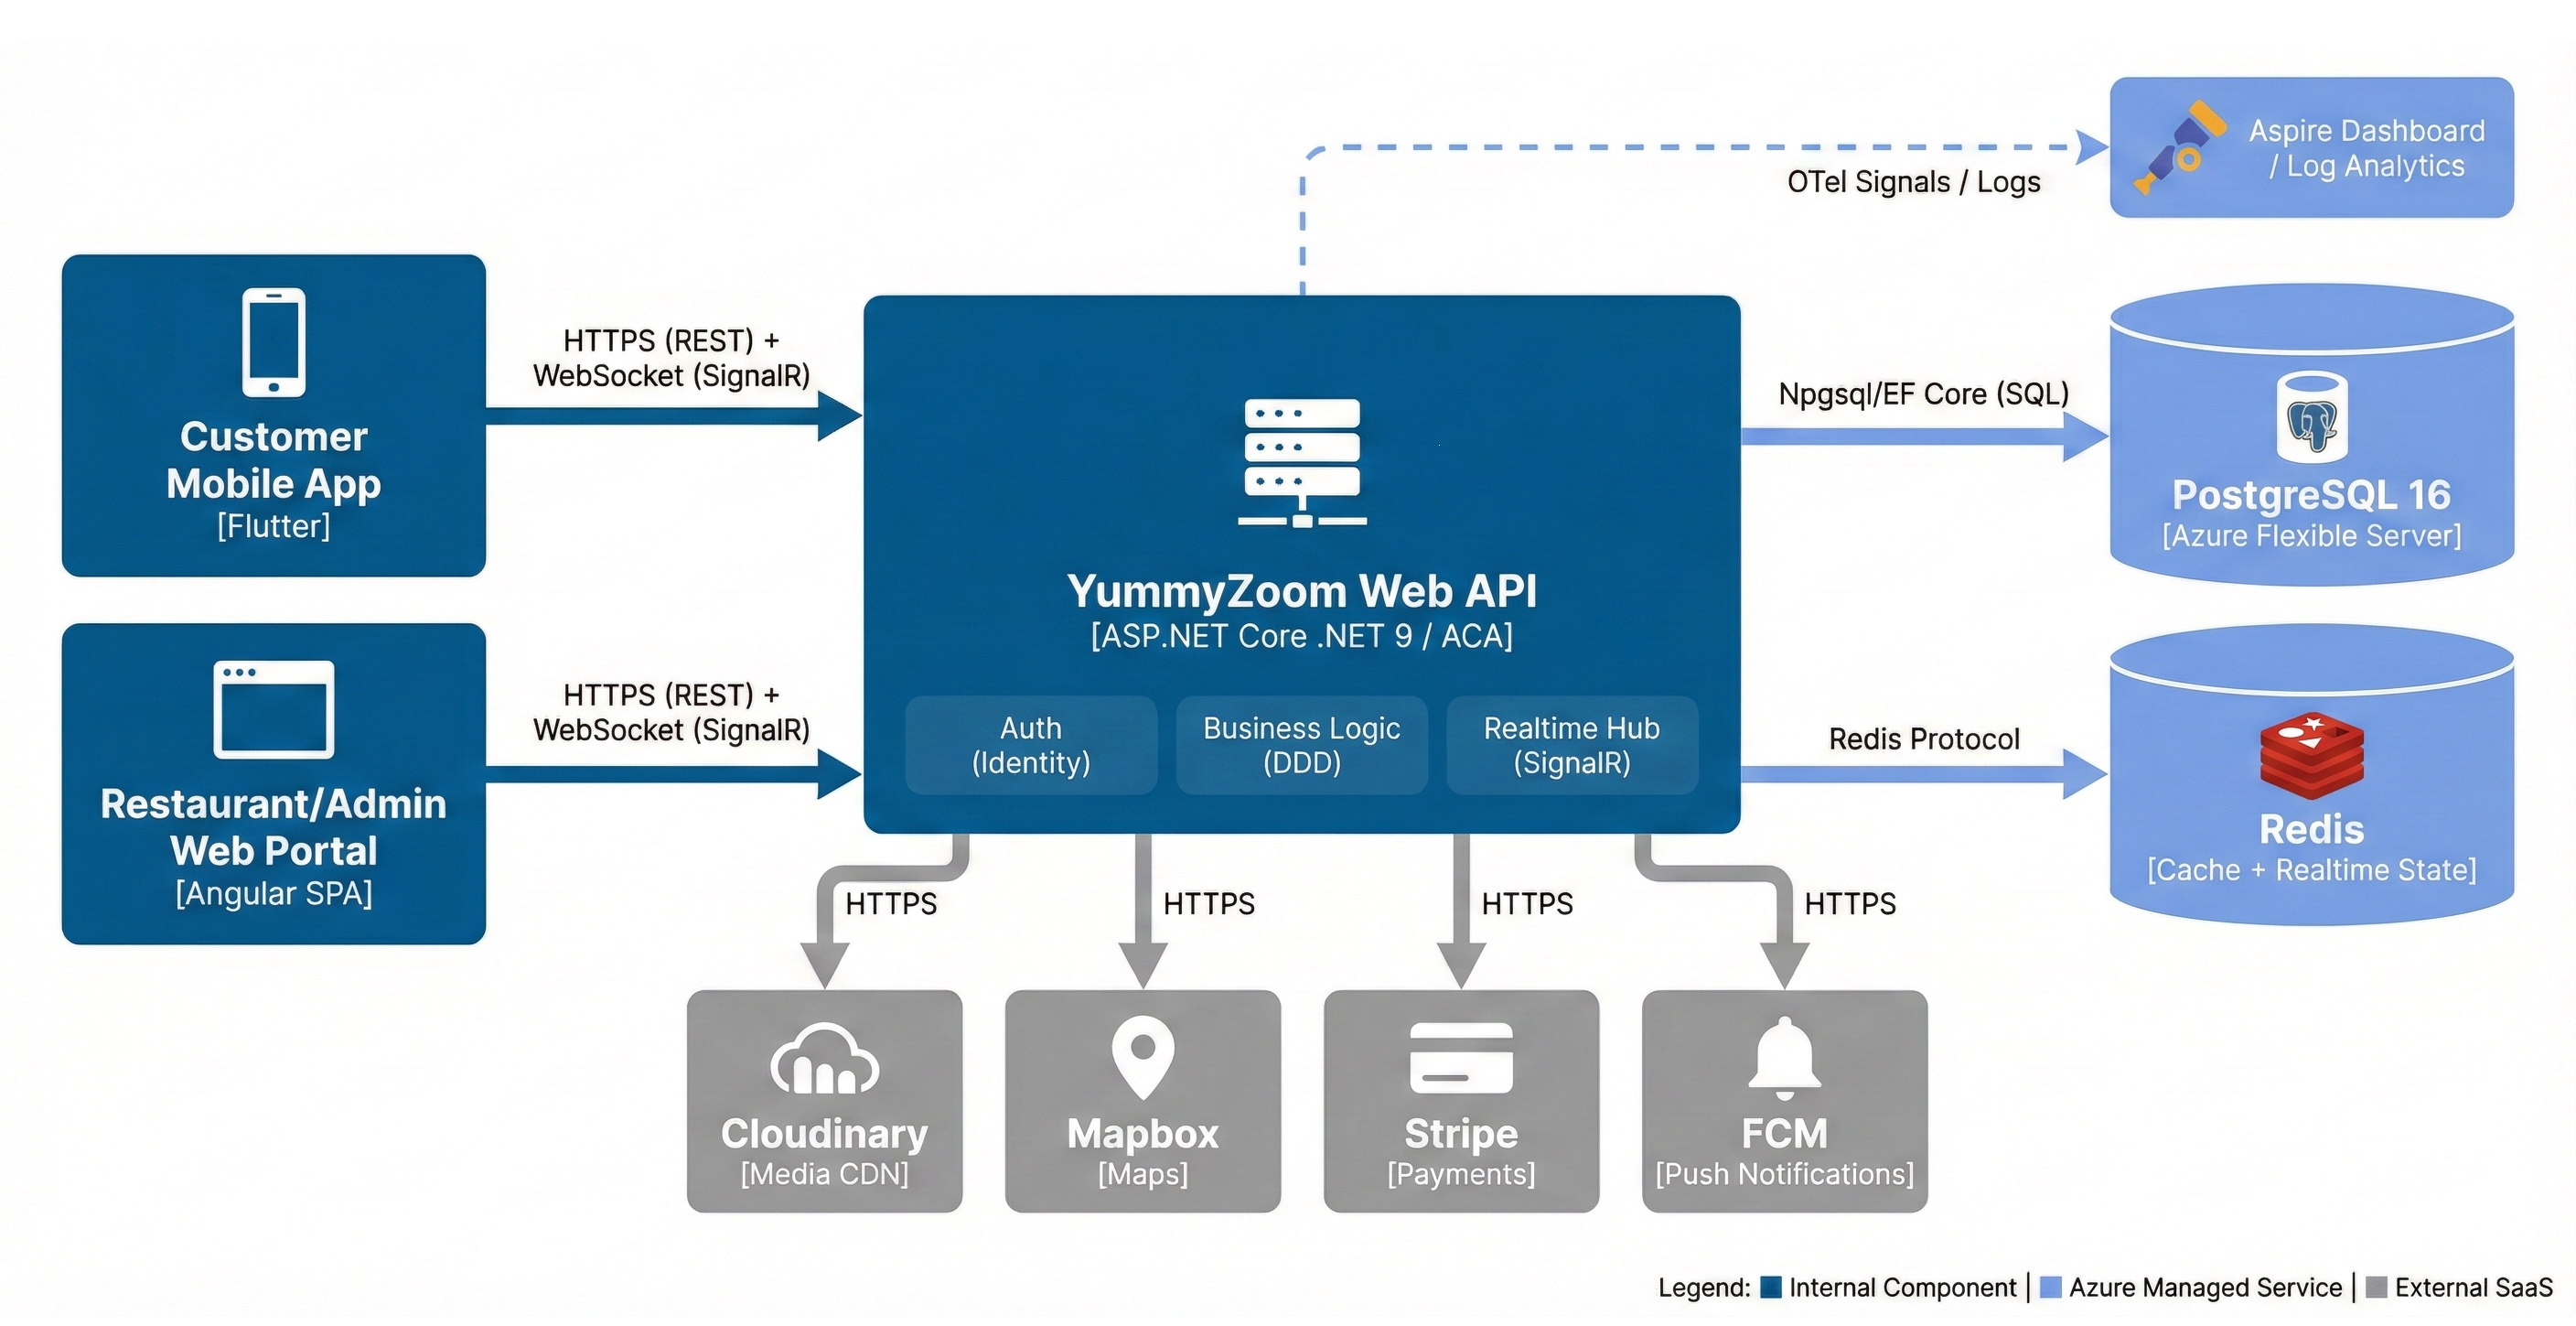
\includegraphics[width=\textwidth]{c4_container_view.png}
    \caption{Sơ đồ kiến trúc hệ thống (C4 Container View)}
    \label{fig:c4-container-view}
\end{figure}

Như thể hiện trong Hình \ref{fig:c4-container-view}, kiến trúc vận hành dựa trên sự phối hợp chặt chẽ giữa bốn nhóm thành phần chính, tạo thành một luồng xử lý khép kín từ người dùng đến dữ liệu và các dịch vụ vệ tinh.

Tại điểm khởi đầu, các Client Apps đóng vai trò là cổng giao tiếp chính. Người dùng cuối truy cập hệ thống thông qua ứng dụng di động đa nền tảng được xây dựng bằng Flutter, trong khi đội ngũ quản trị vận hành hệ thống qua Web Portal phát triển trên Angular. Mọi tương tác của người dùng từ việc lướt danh sách món ăn đến đặt hàng đều được chuyển tải về máy chủ thông qua giao thức HTTPS bảo mật cho các tác vụ Request-Response tiêu chuẩn, hoặc qua kênh WebSocket (SignalR) đối với các tính năng đòi hỏi sự tức thời như theo dõi TeamCart hay nhận thông báo đơn hàng.

Tiếp nhận các yêu cầu này là Khối Backend Core, cốt lõi của hệ thống chạy trên nền tảng .NET 9 ASP.NET Core. Tại đây, các module nghiệp vụ (Business Logic) thực thi các quy tắc cốt lõi của miền ứng dụng Food Delivery, được bảo vệ bởi lớp xác thực tập trung (Identity) nhằm đảm bảo chỉ những yêu cầu hợp lệ mới được xử lý. Bên cạnh đó, Realtime Hub chịu trách nhiệm duy trì hàng nghìn kết nối thời gian thực, đóng vai trò như tháp điều không tin cậy điều phối luồng thông tin giữa các bên tham gia. Mặc dù hệ thống được thiết kế theo định hướng sẵn sàng cho Microservices, trong giai đoạn MVP, đồ án ưu tiên mô hình Modular Monolith để tối ưu hóa chi phí vận hành trên một Azure Container App duy nhất và loại bỏ độ trễ mạng giữa các dịch vụ. Tuy nhiên, nhờ việc áp dụng Clean Architecture và phân tách module nghiêm ngặt, hệ thống có thể được tách thành các vi dịch vụ độc lập một cách dễ dàng khi quy mô người dùng tăng trưởng.

Dữ liệu sau khi xử lý được lưu trữ bền vững tại Tầng Dữ liệu và Tích hợp (Data \& Integration). PostgreSQL 16 với phần mở rộng PostGIS được sử dụng làm kho lưu trữ chính (Primary Store) cho các dữ liệu quan trọng và phức tạp như thông tin địa lý, đơn hàng và danh mục. Song song đó, Redis đóng vai trò là bộ nhớ đệm (Cache) giúp giảm tải cho cơ sở dữ liệu chính và hoạt động như một trục liên lạc (Pub/Sub Bus) để đồng bộ trạng thái giữa các phiên bản ứng dụng khác nhau.

Cuối cùng, để tối ưu hóa nguồn lực và tập trung vào nghiệp vụ cốt lõi, hệ thống tích hợp sâu với Nhóm Dịch vụ bên thứ ba (External SaaS). Quy trình nghiệp vụ thường xuyên gọi đến các dịch vụ này: khi người dùng tìm kiếm quán ăn, Mapbox cung cấp dữ liệu bản đồ số; khi hình ảnh món ăn được tải lên, Cloudinary đảm nhận việc lưu trữ và tối ưu hóa media; khi thanh toán đơn hàng, giao dịch được xử lý an toàn qua Stripe; và khi trạng thái đơn hàng thay đổi, FCM (Firebase Cloud Messaging) sẽ lập tức gửi thông báo đẩy đến thiết bị người dùng, khép lại vòng đời của một luồng nghiệp vụ.

\section{Các thành phần hạ tầng cốt lõi trên Microsoft Azure}

Để hiện thực hóa kiến trúc Cloud Native, đồ án khởi đầu với .NET Aspire - một công cụ điều phối (Orchestrator) có vai trò tương tự như Docker Compose nhưng được tích hợp sâu vào nền tảng .NET. Thay vì phải cấu hình thủ công các file YAML phức tạp để kết nối các thành phần như Web API, Database (PostgreSQL) hay Cache (Redis), Aspire cho phép định nghĩa toàn bộ hệ thống trực tiếp bằng mã nguồn C\#. Điều này giúp đảm bảo sự nhất quán tuyệt đối: cấu trúc ứng dụng chạy trên máy cục bộ của lập trình viên sẽ giống hệt với mô hình được triển khai thực tế trên đám mây.

Hạ tầng Azure được tổ chức xoay quanh Azure Container Apps (ACA), một nền tảng Serverless cho phép chạy các Docker Container mà không cần quan tâm đến máy chủ vật lý hay các cụm Kubernetes phức tạp. Để đảm bảo an toàn, các container này được đặt trong một Azure Container Apps Environment (ACE) - hoạt động như một mạng ảo bảo vệ, cho phép các dịch vụ giao tiếp nội bộ với nhau mà không bị lộ ra Internet công cộng. Các Docker Image của dự án được lưu trữ an toàn trong Azure Container Registry (ACR), đóng vai trò như một Private Docker Hub - nơi quản lý phiên bản và quét mã độc quy tập trung.

Việc quản lý tài nguyên trên Azure được thực hiện bên trong một Resource Group (RG) tập trung, giúp gom nhóm toàn bộ dịch vụ vào một đơn vị quản lý duy nhất để dễ dàng theo dõi chi phí và vòng đời. Về mặt bảo mật, hệ thống loại bỏ hoàn toàn việc lưu trữ mật khẩu trong mã nguồn bằng cách sử dụng Azure Key Vault kết hợp với Managed Identity. Cơ chế này cung cấp cho mỗi dịch vụ một định danh điện tử, cho phép chúng tự động xác thực và truy cập tài nguyên cần thiết một cách an toàn mà không cần can thiệp thủ công. Cuối cùng, Log Analytics Workspace đóng vai trò là trạm quan sát trung tâm, thu thập mọi nhật ký hoạt động từ ứng dụng để phục vụ việc giám sát và gỡ lỗi.


\section{Kiến trúc triển khai điện toán thực tế trên Azure}

Mô hình triển khai thực tế trên Azure (Hình \ref{fig:azure-deployment-view}) tận dụng tối đa các dịch vụ PaaS và Serverless đã nêu trên để giảm thiểu gánh nặng quản trị hạ tầng.

\begin{figure}[H]
    \centering
    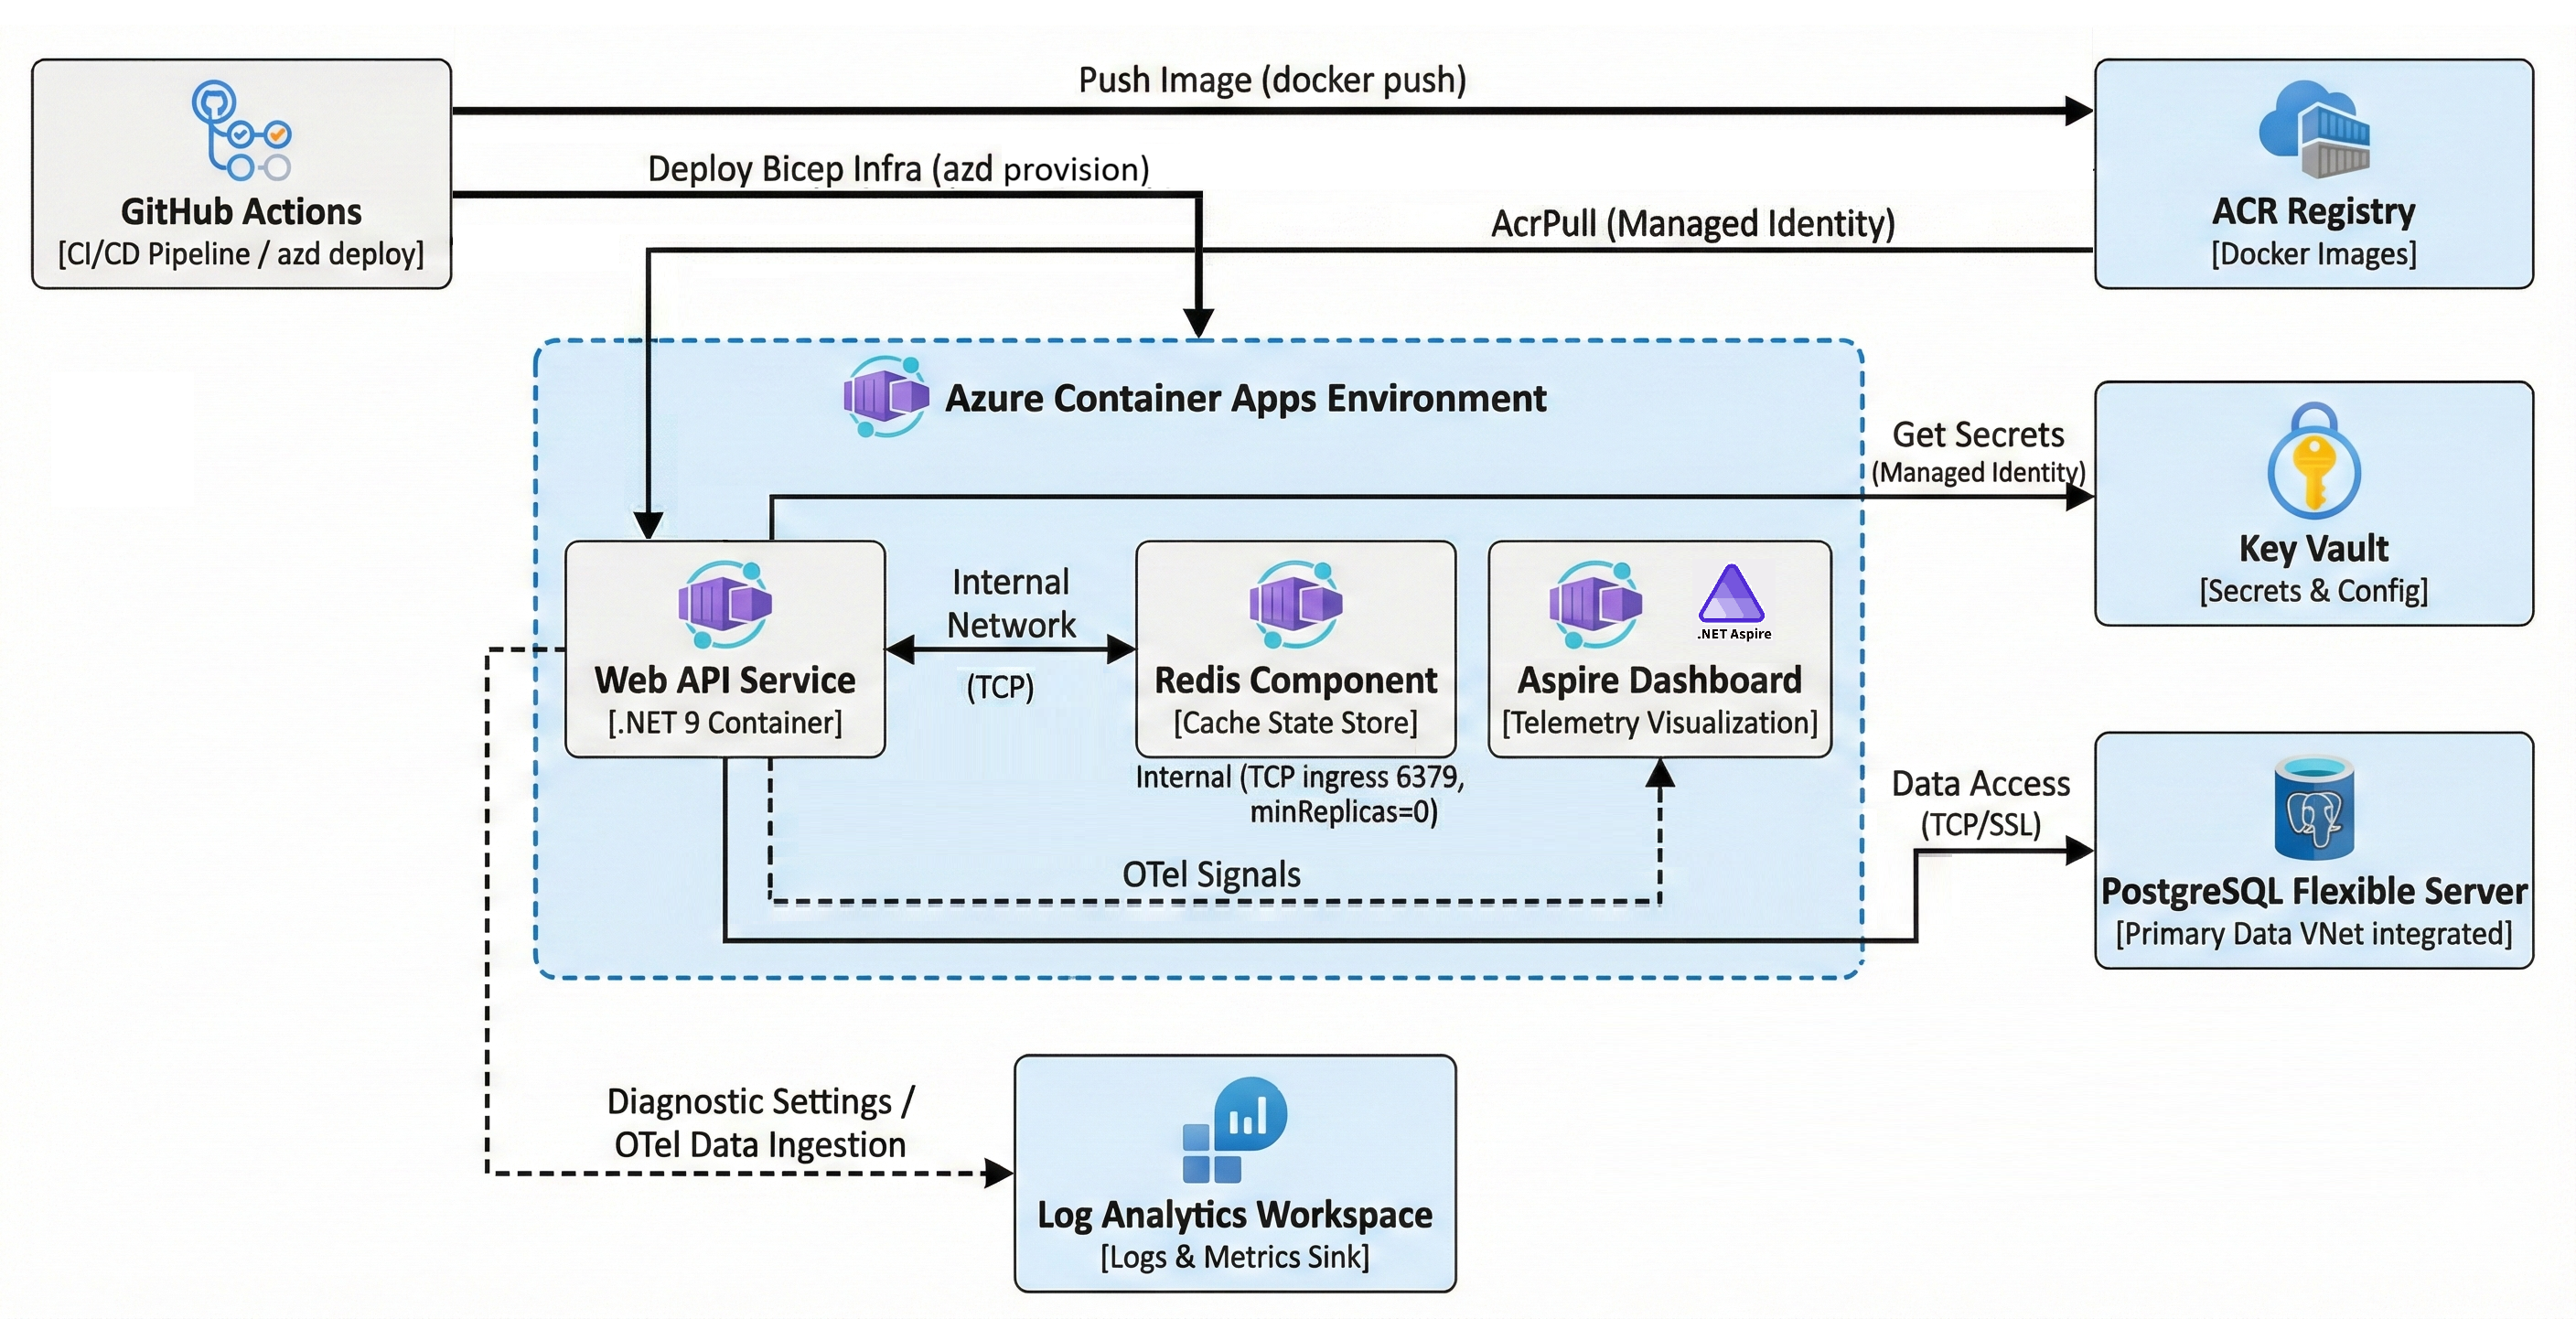
\includegraphics[width=\textwidth]{azure_deployment_view.png}
    \caption{Sơ đồ triển khai vật lý trên Microsoft Azure}
    \label{fig:azure-deployment-view}
\end{figure}

Quan sát Hình \ref{fig:azure-deployment-view}, luồng triển khai và vận hành được liên kết chặt chẽ thông qua các thành phần hạ tầng cốt lõi. Trung tâm của hệ thống là Azure Container Apps Environment, nơi lưu trữ và vận hành ba thành phần chính: Web API Service (.NET 9) đóng vai trò xử lý yêu cầu, Redis Component cung cấp bộ nhớ đệm nội bộ qua giao thức TCP, và Aspire Dashboard tiếp nhận các tín hiệu OTel (OpenTelemetry) để trực quan hóa trạng thái sức khỏe của ứng dụng.

Về mặt tích hợp dữ liệu và bảo mật, Web API kết nối tới PostgreSQL Flexible Server thông qua giao thức TCP/SSL để truy xuất dữ liệu bền vững. Các thông tin nhạy cảm (Secrets) được quản lý tập trung tại Key Vault và chỉ được truy cập thông qua cơ chế Managed Identity, đảm bảo nguyên tắc không lưu trữ mật khẩu trong mã nguồn. Tương tự, Managed Identity cũng cấp quyền để Container App kéo (Pull) các Image mới nhất từ ACR Registry.

Toàn bộ quy trình trên được điều phối tự động bởi GitHub Actions. Pipeline CI/CD thực hiện song song hai nhiệm vụ: đóng gói và đẩy Container Image lên ACR, đồng thời sử dụng Bicep (thông qua lệnh \texttt{azd provision}) để cung cấp tài nguyên hạ tầng. Cuối cùng, mọi dữ liệu nhật ký và số liệu giám sát từ môi trường chạy đều được đẩy về Log Analytics Workspace, tạo thành một vòng lặp DevSecOps khép kín và an toàn. Chi tiết về quy trình pipeline sẽ được trình bày trong Chương \ref{chap:devops-cicd}.

\section{Phân tích và so sánh kiến trúc}

Các quyết định công nghệ quan trọng được tóm tắt trong Bảng \ref{tab:adr-analysis}, cân bằng giữa hiệu quả chi phí và khả năng mở rộng.

\begin{table}[H]
    \centering
    \caption{Phân tích quyết định kiến trúc (ADR)}
    \label{tab:adr-analysis}
    \begin{tabular}{|p{0.2\linewidth}|p{0.25\linewidth}|p{0.45\linewidth}|}
        \hline
        \textbf{Hạng mục} & \textbf{Lựa chọn} & \textbf{Lý do chính} \\
        \hline
        Compute & Container Apps & Serverless, không cần quản lý Kubernetes Cluster phức tạp. \\
        \hline
        Database & Postgres Flexible & Tối ưu cho dữ liệu địa lý (PostGIS), chi phí thấp hơn SQL Server. \\
        \hline
        IaC & Azure Bicep & Cú pháp đơn giản, tích hợp sâu vào quy trình Azure CLI. \\
        \hline
    \end{tabular}
\end{table}

Đáng chú ý trong lựa chọn công nghệ IaC, đồ án ưu tiên sử dụng Azure Bicep thay vì Terraform. Mặc dù Terraform có lợi thế về đa nền tảng, Bicep được chọn nhờ khả năng tích hợp native với Azure, loại bỏ gánh nặng quản lý tệp trạng thái (state file) phức tạp và tận dụng tối đa sự hỗ trợ từ công cụ Azure Developer CLI (azd) để đơn giản hóa quy trình triển khai.

So với mô hình máy ảo (VM) truyền thống, kiến trúc này loại bỏ hoàn toàn việc cấu hình thủ công OS/Runtime và vá lỗi bảo mật (patching). Thời gian khởi tạo tài nguyên giảm từ vài phút xuống vài giây, và việc cập nhật ứng dụng diễn ra không gián đoạn (Zero Downtime) nhờ cơ chế Revisions của Container Apps.

\section*{Kết chương}
Chương này đã giới thiệu kiến trúc tổng thể dưới góc nhìn logic và vật lý, làm nền tảng cho các nội dung chi tiết về mã hóa hạ tầng (IaC) sẽ được trình bày trong chương kế tiếp.


% ==================================================

\chapter{Hạ tầng dưới dạng mã (IaC): azd + Bicep + Azure Container Apps}

Chương này đi sâu vào phương pháp "Hạ tầng dưới dạng mã" (Infrastructure as Code - IaC) mà đồ án áp dụng để định nghĩa và quản lý tài nguyên trên Azure. Thay vì thao tác thủ công trên giao diện Azure Portal là cách làm dễ gây lỗi và khó tái lập, đồ án sử dụng bộ công cụ hiện đại gồm .NET Aspire, Bicep và Azure Developer CLI (azd) để tự động hóa hoàn toàn quy trình này.

\section{Vai trò của .NET Aspire AppHost trong định nghĩa hạ tầng}

Trong kiến trúc truyền thống, mã nguồn ứng dụng (C\#) và mã nguồn hạ tầng (Terraform/YAML) thường bị tách biệt, dẫn đến sự thiếu đồng bộ. .NET Aspire giải quyết vấn đề này bằng cách đưa định nghĩa hạ tầng vào ngay trong code C\# thông qua dự án \texttt{AppHost}.

Về mặt nguyên lý, \texttt{AppHost} đóng vai trò là "Nguồn chân lý" (Source of Truth) cho kiến trúc logic. Nó định nghĩa các thành phần của hệ thống và mối quan hệ giữa chúng. Tại đây, đồ án tận dụng tính năng "mô hình hóa tài nguyên" của Aspire để tạo ra sự tương đồng giữa môi trường phát triển (Dev) và sản phẩm (Production).

Ví dụ, đối với dịch vụ Redis:
\begin{itemize}
    \item \textbf{Môi trường Dev}: Khi chạy cục bộ, lệnh \texttt{AddRedis("redis")} sẽ tự động kéo Docker Image của Redis về và chạy một container tạm thời.
    \item \textbf{Môi trường Production}: Khi triển khai, Aspire hiểu rằng tài nguyên này ánh xạ tới một dịch vụ Redis thực thụ trên Azure. Cụ thể trong đồ án này, nó được ánh xạ tới một Azure Container App chạy Redis image thông qua phương thức \texttt{AddConnectionString("redis")}.
\end{itemize}

Đoạn mã sau trong \texttt{Program.cs} minh họa logic phân tách môi trường này:

\begin{lstlisting}[language={[Sharp]C}, caption={Cấu hình Dev/Prod Parity trong AppHost}, label={code:apphost-parity}]
var isPublishMode = builder.ExecutionContext.IsPublishMode;

if (isPublishMode) {
    // Production: Azure Database for PostgreSQL
    var postgres = builder.AddAzurePostgresFlexibleServer("postgres");
} else {
    // Development: Local Container
    var postgres = builder.AddPostgres("postgres")
        .WithImage("postgis/postgis", "16-3.4") // PostGIS support
        .WithPgAdmin();
}
\end{lstlisting}

Cách tiếp cận này mang lại lợi ích kép: vừa giúp lập trình viên kiểm soát kiến trúc ngay tại thời điểm biên dịch (Compile-time check), vừa đảm bảo môi trường Dev phản ánh chính xác cấu trúc của hệ thống thật.

\section{Kiến trúc Bicep Modules và Tài nguyên Azure}

Đồ án sử dụng ngôn ngữ Bicep để mô tả chi tiết các tài nguyên vật lý trên Azure. Các file Bicep được tổ chức thành các module nhỏ gọn, nằm trong thư mục \texttt{src/AppHost/infra/}, giúp dễ dàng quản lý và tái sử dụng.

\subsection{Tài nguyên nền tảng (Shared Resources)}

Module \texttt{resources.bicep} chịu trách nhiệm khởi tạo các thành phần nền tảng dùng chung cho toàn bộ hệ thống. Thay vì chỉ liệt kê các dịch vụ, module này tập trung vào việc thiết lập sự liên kết chặt chẽ giữa chúng. Cụ thể, Azure Container Apps Environment được cấu hình với Profile \texttt{Consumption} để đảm bảo tính tối ưu về chi phí, chỉ tính phí dựa trên tài nguyên thực tế sử dụng. Đồng thời, toàn bộ nhật ký và chỉ số vận hành được định hướng tập trung về Log Analytics Workspace. Để đảm bảo an ninh, một định danh duy nhất (User Assigned Managed Identity) được khởi tạo và gán cho các dịch vụ, cho phép Web API có thể kéo Docker Image từ ACR mà không cần sử dụng mật khẩu.

\subsection{Tài nguyên dữ liệu (Data Resources)}

Các tài nguyên phục vụ lưu trữ được định nghĩa riêng biệt để đảm bảo tính cô lập và an toàn dữ liệu cao nhất. Đối với PostgreSQL Flexible Server, đồ án áp dụng SKU \texttt{Standard\_B1ms} (dòng Burstable) nhằm cân bằng giữa hiệu năng xử lý và ngân sách của giai đoạn MVP, với dung lượng lưu trữ khởi tạo 32GB. Một điểm quan trọng trong cấu hình này là việc tự động kích hoạt các tiện ích mở rộng như \texttt{postgis}, \texttt{pg\_trgm} và \texttt{unaccent} ngay tại thời điểm cấp phát tài nguyên thông qua Bicep, giúp hệ thống sẵn sàng xử lý các yêu cầu nghiệp vụ phức tạp về tìm kiếm và vị trí địa lý.

Đối với bộ nhớ đệm, thay vì sử dụng dịch vụ Azure Redis Cache độc lập vốn có chi phí duy trì cao, đồ án thực hiện triển khai Redis trực tiếp dưới dạng một thành phần (Component) trong môi trường Container Apps. Cách tiếp cận này giúp Redis giao tiếp với Web API hoàn toàn qua mạng nội bộ của ACE, vừa tăng cường bảo mật vừa tiết kiệm đáng kể chi phí vận hành mà vẫn đảm bảo được hiệu năng cần thiết.


Cấu hình Bicep dưới đây (`postgres.module.bicep`) cho thấy cách tài nguyên được định nghĩa chi tiết, bao gồm cả phiên bản và các tiện ích mở rộng:

\begin{lstlisting}[language=Python, caption={Định nghĩa tài nguyên PostgreSQL với Bicep}, label={code:bicep-postgres}]
resource postgres 'Microsoft.DBforPostgreSQL/flexibleServers@2024-08-01' = {
  name: take('postgres-${uniqueString(resourceGroup().id)}', 63)
  sku: {
    name: 'Standard_B1ms' // Cost-optimized SKU
    tier: 'Burstable'
  }
  properties: {
    version: '16'
    storage: { storageSizeGB: 32 }
  }
}

resource postgresExtensions 'Microsoft.DBforPostgreSQL/flexibleServers/configurations@2024-08-01' = {
  name: 'azure.extensions'
  parent: postgres
  properties: { value: 'postgis,pg_trgm,unaccent' }
}
\end{lstlisting}

\subsection{Aspire Dashboard}
Thành phần Dashboard giám sát được triển khai như một \texttt{.NET Component} ngay trong môi trường Container Apps. Nó tiếp nhận các tín hiệu OTel (Logs, Traces, Metrics) từ Web API, cung cấp giao diện trực quan để theo dõi sức khỏe hệ thống theo thời gian thực.

\section{Quy trình cấp phát với Azure Developer CLI (azd)}

Công cụ \texttt{azd} đóng vai trò là "nhạc trưởng" điều phối toàn bộ quy trình cấp phát và triển khai. File cấu hình \texttt{azure.yaml} định nghĩa dự án và liên kết code với hạ tầng.

Quy trình triển khai tiêu chuẩn diễn ra qua các bước:
\begin{enumerate}
    \item \textbf{azd provision}: Lệnh này phân tích các file Bicep, so sánh trạng thái mong muốn với thực tế trên Azure, và thực hiện cấp phát hoặc cập nhật tài nguyên lên nền tảng Azure. 
    \item \textbf{State Management}: \texttt{azd} quản lý trạng thái môi trường (như Resource ID) trong thư mục \texttt{.azure/}. Các biến môi trường nhạy cảm được lưu trong file \texttt{.env} và tự động liên kết (binding) vào tham số của Bicep khi chạy lệnh.
\end{enumerate}

\section{Chiến lược Quản lý Bảo mật và Cấu hình}

Đồ án áp dụng triệt để mô hình bảo mật Zero Trust, tập trung vào việc loại bỏ hoàn toàn các thông tin nhạy cảm khỏi mã nguồn. Thay vì sử dụng mật khẩu tĩnh hay chuỗi kết nối thủ công vốn tiềm ẩn nhiều rủi ro rò rỉ, hệ thống tận dụng sự phối hợp tự động giữa Managed Identity và Azure Key Vault.

Quy trình quản lý bảo mật được thiết kế khép kín bắt đầu từ giai đoạn cấp phát hạ tầng. Module \texttt{keyvault.module.bicep} khởi tạo kho lưu trữ bí mật với các chính sách truy cập (RBAC) nghiêm ngặt. Trong quá trình triển khai, các giá trị nhạy cảm như mật khẩu quản trị PostgreSQL hay khóa truy cập các dịch vụ bên thứ ba được sinh ra động và lưu trữ trực tiếp vào Key Vault thông qua module \texttt{keyvault-secrets.module.bicep}. 

Tại thời điểm ứng dụng khởi động, Web API sử dụng Managed Identity được gán sẵn để tự xác thực và truy xuất các cấu hình cần thiết từ Key Vault mà không cần bất kỳ thông tin đăng nhập nào được lưu trong code. Cơ chế này đảm bảo an toàn tối đa cho môi trường Production, đồng thời giúp đội ngũ phát triển không cần tiếp xúc trực tiếp với các bí mật hệ thống, từ đó giảm thiểu rủi ro bảo mật từ yếu tố con người.


\section*{Kết chương}

Chương này đã trình bày chi tiết cách thức hiện thực hóa kiến trúc hệ thống thông qua mã nguồn, từ việc định nghĩa logic trong AppHost đến cấp phát tài nguyên vật lý bằng Bicep và azd. Việc áp dụng các chuẩn mực bảo mật như Managed Identity và Key Vault cũng được phân tích cụ thể. Chương tiếp theo sẽ mô tả quy trình tích hợp và triển khai liên tục (CI/CD) để tự động hóa vòng đời phát triển này.

% ==================================================

\chapter{Quy trình phát triển và Vận hành (DevOps và CI/CD)}
\label{chap:devops-cicd}

Chương này trình bày quy trình tích hợp và triển khai liên tục (CI/CD) được áp dụng trong dự án, tập trung vào việc tự động hóa vòng đời phát triển từ khi lập trình viên đẩy mã nguồn lên kho lưu trữ cho đến khi ứng dụng sẵn sàng phục vụ người dùng trên nền tảng Azure. Quá trình này được hiện thực hóa thông qua sự kết hợp giữa GitHub Actions và công cụ Azure Developer CLI (azd).

\section{Tổng quan quy trình CI/CD}

Đồ án thiết lập một pipeline thống nhất để quản lý cả mã nguồn ứng dụng và mã nguồn hạ tầng (IaC). Thay vì tách rời hai quy trình này, việc tích hợp chúng đảm bảo tính nhất quán của môi trường: hạ tầng luôn được cập nhật tương ứng với phiên bản mã nguồn mới nhất.

Quá trình triển khai tự động diễn ra theo trình tự sau:
\begin{enumerate}
    \item Lập trình viên hoàn tất tính năng và đẩy mã nguồn (Push Code) lên nhánh chính \texttt{main} trên GitHub.
    \item GitHub Actions tự động kích hoạt pipeline (Workflow).
    \item Pipeline thực hiện xác thực với Azure sử dụng cơ chế OpenID Connect (OIDC).
    \item Công cụ \texttt{azd} đồng bộ hóa trạng thái hạ tầng thực tế với định nghĩa trong mã Bicep (Provision).
    \item Sau khi hạ tầng sẵn sàng, \texttt{azd} thực hiện đóng gói ứng dụng thành Container Image và triển khai phiên bản mới lên Azure Container Apps (Deploy).
\end{enumerate}

Hình \ref{fig:cicd-flow} dưới đây minh họa luồng đi của dữ liệu và các bước xử lý chính trong pipeline.

\begin{figure}[H]
    \centering
    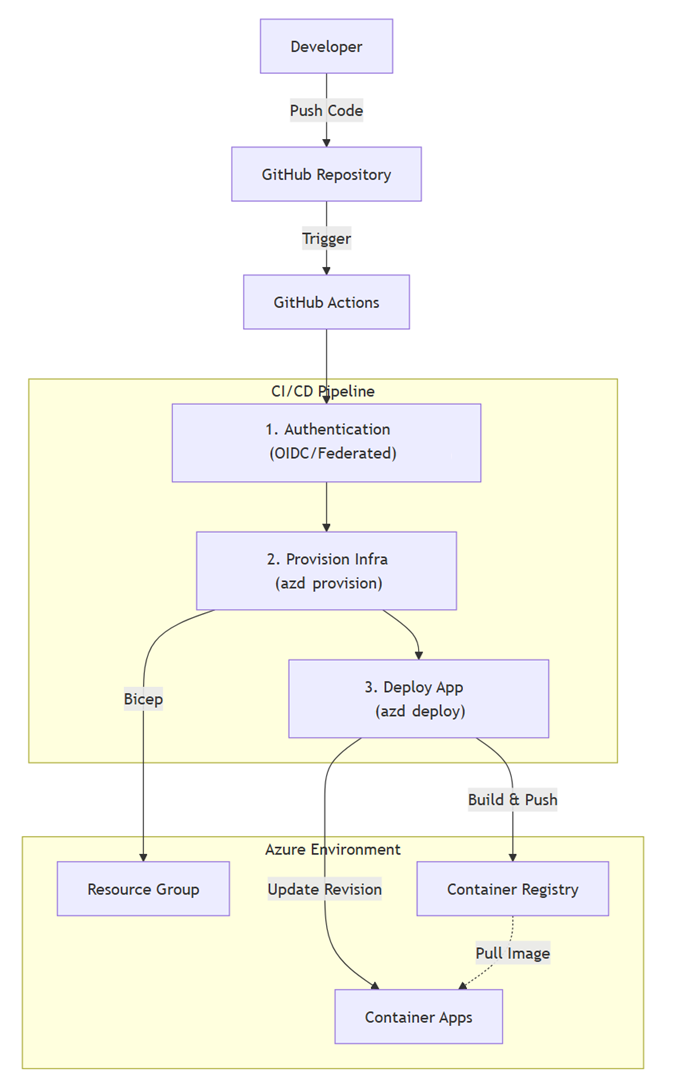
\includegraphics[width=0.9\linewidth]{cicd-flow}
    \caption{Sơ đồ luồng Tích hợp và Triển khai liên tục (CI/CD)}
    \label{fig:cicd-flow}
\end{figure}

\section{Cơ chế Bảo mật và Xác thực không mật khẩu (Secretless)}

Một trong những hạn chế của các phương pháp CI/CD truyền thống là việc phải lưu trữ thông tin đăng nhập (như Client Secret của Service Principal) trên kho chứa mã nguồn hoặc biến môi trường của CI. Điều này tiềm ẩn rủi ro rò rỉ và đòi hỏi công sức quản lý việc xoay vòng mật khẩu định kỳ.

Đồ án giải quyết vấn đề này bằng cách áp dụng cơ chế xác thực OpenID Connect (OIDC) với Federated Credentials. Trong mô hình này, GitHub Actions đóng vai trò là một định danh (Identity) được Azure tin tưởng. Khi pipeline chạy, GitHub cấp một token ngắn hạn, và Azure xác thực token này để cấp quyền truy cập tạm thời vào tài nguyên.

Nhờ đó, đồ án đạt được tiêu chí "Zero Trust" ngay trong khâu triển khai: không có bất kỳ mật khẩu dài hạn (Long-lived secret) nào được lưu trữ.

\section{Chi tiết luồng thực thi (Workflow Implementation)}

File cấu hình \texttt{.github/workflows/azure-dev.yml} định nghĩa chi tiết các bước thực thi của pipeline. Dưới đây là phân tích các giai đoạn quan trọng:

\subsection{Khởi tạo và Xác thực}
Trước tiên, môi trường CI được thiết lập với các công cụ cần thiết như .NET SDK và \texttt{azd}. Sau đó, bước xác thực được thực hiện thông qua \texttt{azd auth login} kết hợp với provider GitHub:

\begin{lstlisting}[language=bash, caption={Xác thực sử dụng Federated Credentials}, label={code:auth-federated}]
- name: Log in with Azure
  run: |
    azd auth login `
      --client-id "$Env:AZURE_CLIENT_ID" `
      --federated-credential-provider "github" `
      --tenant-id "$Env:AZURE_TENANT_ID"
\end{lstlisting}

\subsection{Cấp phát hạ tầng (Provisioning)}
Lệnh \texttt{azd provision} đảm nhận việc triển khai mã nguồn Bicep bằng cách tương tác trực tiếp với nền tảng Azure để quản trị vòng đời của các tài nguyên hạ tầng. Quá trình này tự động hóa việc khởi tạo các dịch vụ cốt lõi như Resource Group, Azure Container Registry, Azure Container Apps, và các thành phần đã được phân tích ở Chương \ref{chap:arch}. Trong trường hợp các tài nguyên này chưa tồn tại, \texttt{azd} sẽ thực hiện cấp phát mới; ngược lại, nếu đã có sẵn, công cụ sẽ tiến hành so sánh và cập nhật các thông số cấu hình để đồng bộ hóa với phiên bản mã nguồn Bicep mới nhất. Bên cạnh đó, hệ thống còn tận dụng cơ chế tự động liên kết (binding) các bí mật từ GitHub Secrets vào tham số của Bicep, giúp các thông tin nhạy cảm như mật khẩu quản trị cơ sở dữ liệu được truyền tải an toàn mà không hiển thị dưới dạng văn bản rõ trong log của pipeline.

\subsection{Đóng gói và Triển khai (Build \& Deploy)}
Giai đoạn cuối cùng là lệnh \texttt{azd deploy}. Tại bước này, \texttt{azd} thực hiện một chuỗi các tác vụ phức tạp:
\begin{enumerate}
    \item Dựa vào Dockerfile hoặc cấu hình mặc định của .NET SDK để đóng gói ứng dụng Web API thành Docker Image.
    \item Đẩy (Push) image này lên Azure Container Registry (ACR) riêng của dự án.
    \item Ra lệnh cho Azure Container Apps cập nhật phiên bản (Revision) mới, trỏ tới image vừa được đẩy lên.
\end{enumerate}

Với cơ chế này, hệ thống hỗ trợ khả năng Zero-Downtime Deployment: Container Apps sẽ khởi động revision mới song song với phiên bản cũ, và chỉ chuyển hướng traffic sang phiên bản mới khi nó đã sẵn sàng (thông qua Health Probes).

\section*{Kết chương}

Chương này đã trình bày quy trình CI/CD tự động hóa hoàn toàn từ mã nguồn đến môi trường Cloud, với điểm nhấn là việc loại bỏ quản lý secret thủ công nhờ OIDC. Việc kết hợp chặt chẽ giữa quy trình cấp phát (Provision) và triển khai (Deploy) trong cùng một pipeline giúp đảm bảo tính nhất quán của hệ thống. Chương tiếp theo sẽ đi sâu vào khía cạnh vận hành, bao gồm giám sát và tối ưu hóa hệ thống sau khi triển khai.

% ==================================================

\chapter{Vận hành, quan sát hệ thống và mở rộng}

Chương này đi sâu vào khía cạnh vận hành của hệ thống sau khi triển khai, tập trung vào khả năng quan sát (Observability), quản lý cấu hình và chiến lược mở rộng (Scaling) để tối ưu hóa chi phí cho giai đoạn MVP.

\section{Kiến trúc Quan sát (Observability Architecture)}

Để đảm bảo khả năng giám sát toàn diện, đồ án áp dụng tiêu chuẩn OpenTelemetry (OTel) làm nền tảng cốt lõi cho việc thu thập dữ liệu vận hành. Thay vì phụ thuộc vào các SDK riêng lẻ của từng nhà cung cấp (như Application Insights SDK), việc sử dụng OTel giúp hệ thống không bị khóa chặt (lock-in) vào một công cụ cụ thể và dễ dàng chuyển hướng dữ liệu khi cần.

Hệ thống thu thập đầy đủ ba trụ cột của Observability:
\begin{itemize}
    \item Logs (Nhật ký): Ghi lại các sự kiện rời rạc xảy ra trong ứng dụng.
    \item Metrics (Chỉ số): Các số liệu định lượng theo thời gian (ví dụ: CPU, RAM, số lượng request/giây).
    \item Traces (Truy vết): Theo dõi hành trình của một yêu cầu (Request) đi qua nhiều service khác nhau.
\end{itemize}

Luồng dữ liệu được thiết kế như sau: Dữ liệu từ Web API được đẩy trực tiếp tới Aspire Dashboard thông qua giao thức OTLP để giám sát thời gian thực. Đồng thời, trên môi trường Azure, các Log và Metric được cấu hình (Diagnostic Settings) để lưu trữ dài hạn vào Log Analytics Workspace.

\section{Giám sát thời gian thực với Aspire Dashboard}

.NET Aspire Dashboard là công cụ mạnh mẽ giúp đội ngũ phát triển và vận hành nắm bắt "mạch đập" của hệ thống ngay lập tức mà không cần cấu hình phức tạp.

\subsection{Theo dõi tài nguyên (Resources)}
Giao diện Resources cung cấp cái nhìn tổng quan về tất cả các thành phần trong hệ thống, bao gồm Web API, Redis Cache, và PostgreSQL. Tại đây, trạng thái hoạt động (Running/Exited), các biến môi trường và endpoint của từng container được hiển thị rõ ràng.

\begin{figure}[H]
    \centering
    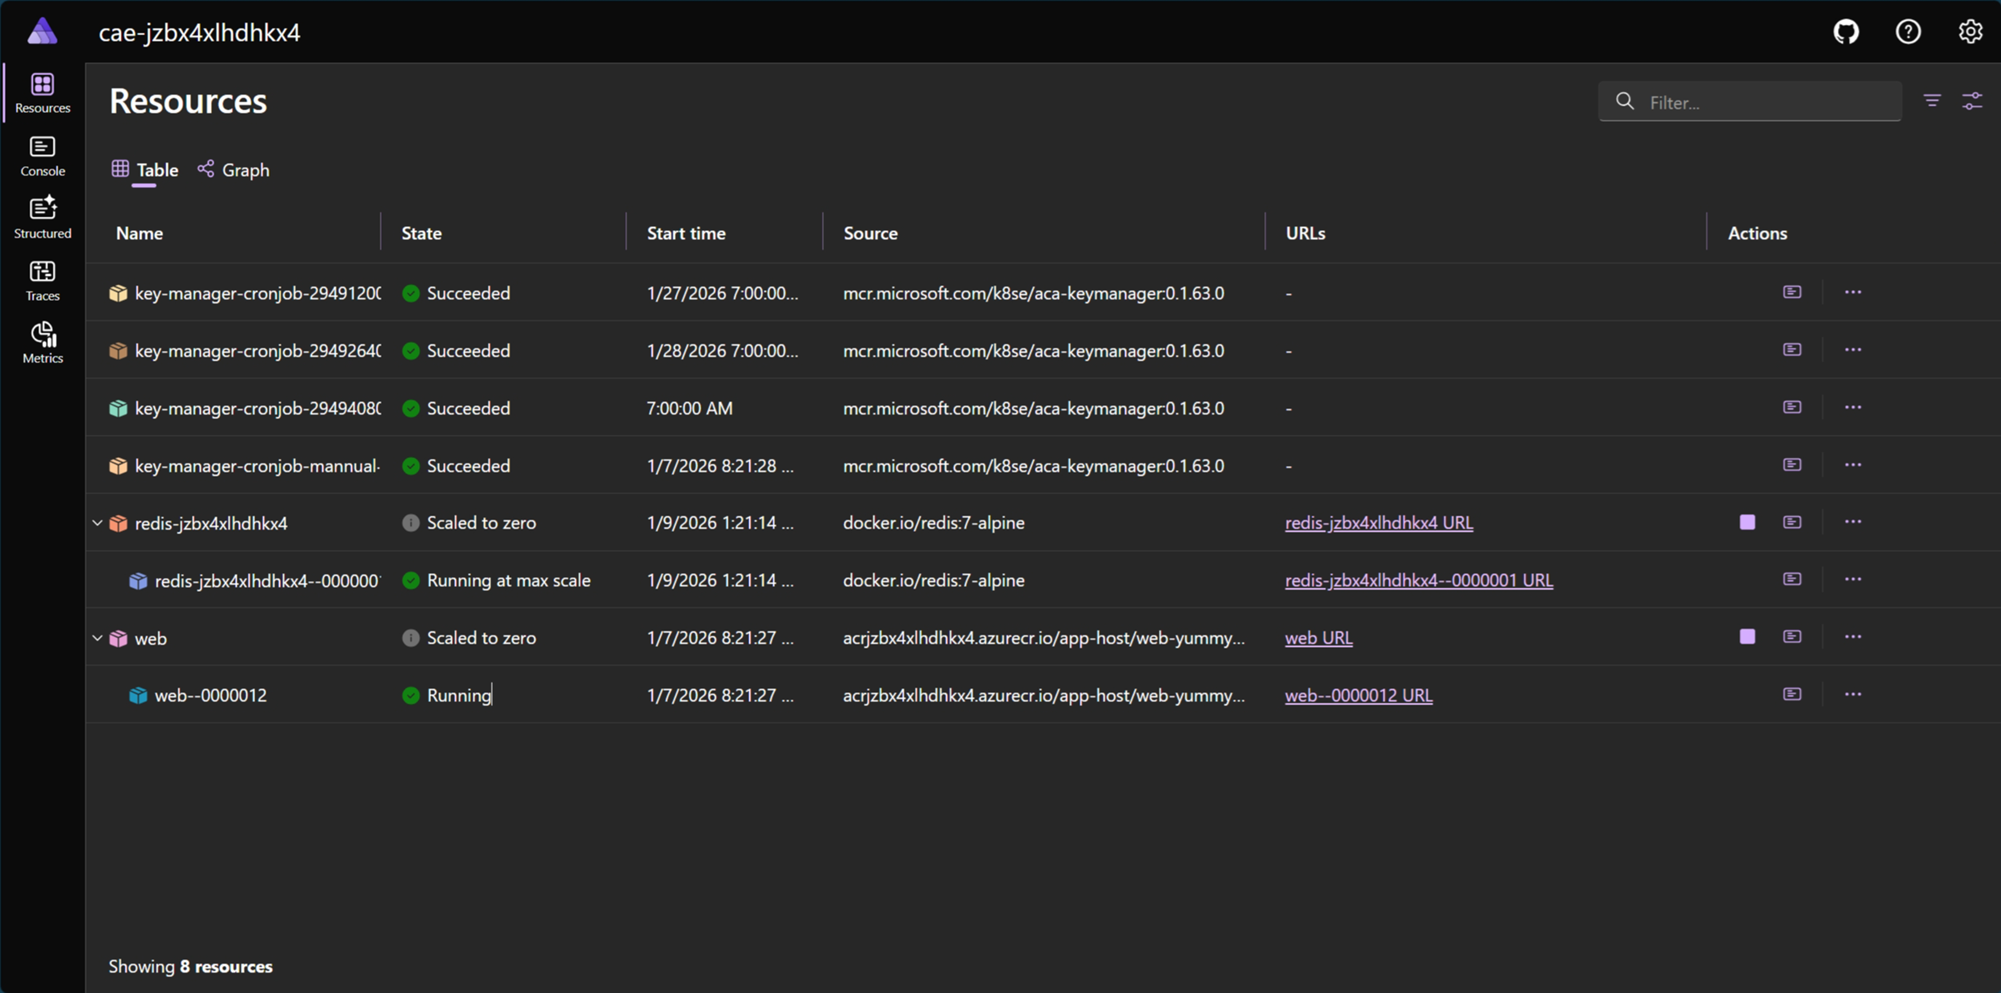
\includegraphics[width=0.95\linewidth]{Dashboard-Resources}
    \caption{Giao diện Resources trên Aspire Dashboard hiển thị các container đang chạy}
    \label{fig:dashboard-resources}
\end{figure}

\subsection{Truy vết phân tán (Distributed Tracing)}
Một trong những tính năng hữu ích nhất là khả năng truy vết (Tracing). Hình \ref{fig:dashboard-traces} và \ref{fig:dashboard-traces-detail} minh họa chi tiết đường đi của một request. Nhờ đó, lập trình viên có thể dễ dàng phát hiện điểm nghẽn cổ chai (bottleneck) hay nguyên nhân gây lỗi (như truy vấn SQL chậm hoặc kết nối Redis bị timeout).

\begin{figure}[H]
    \centering
    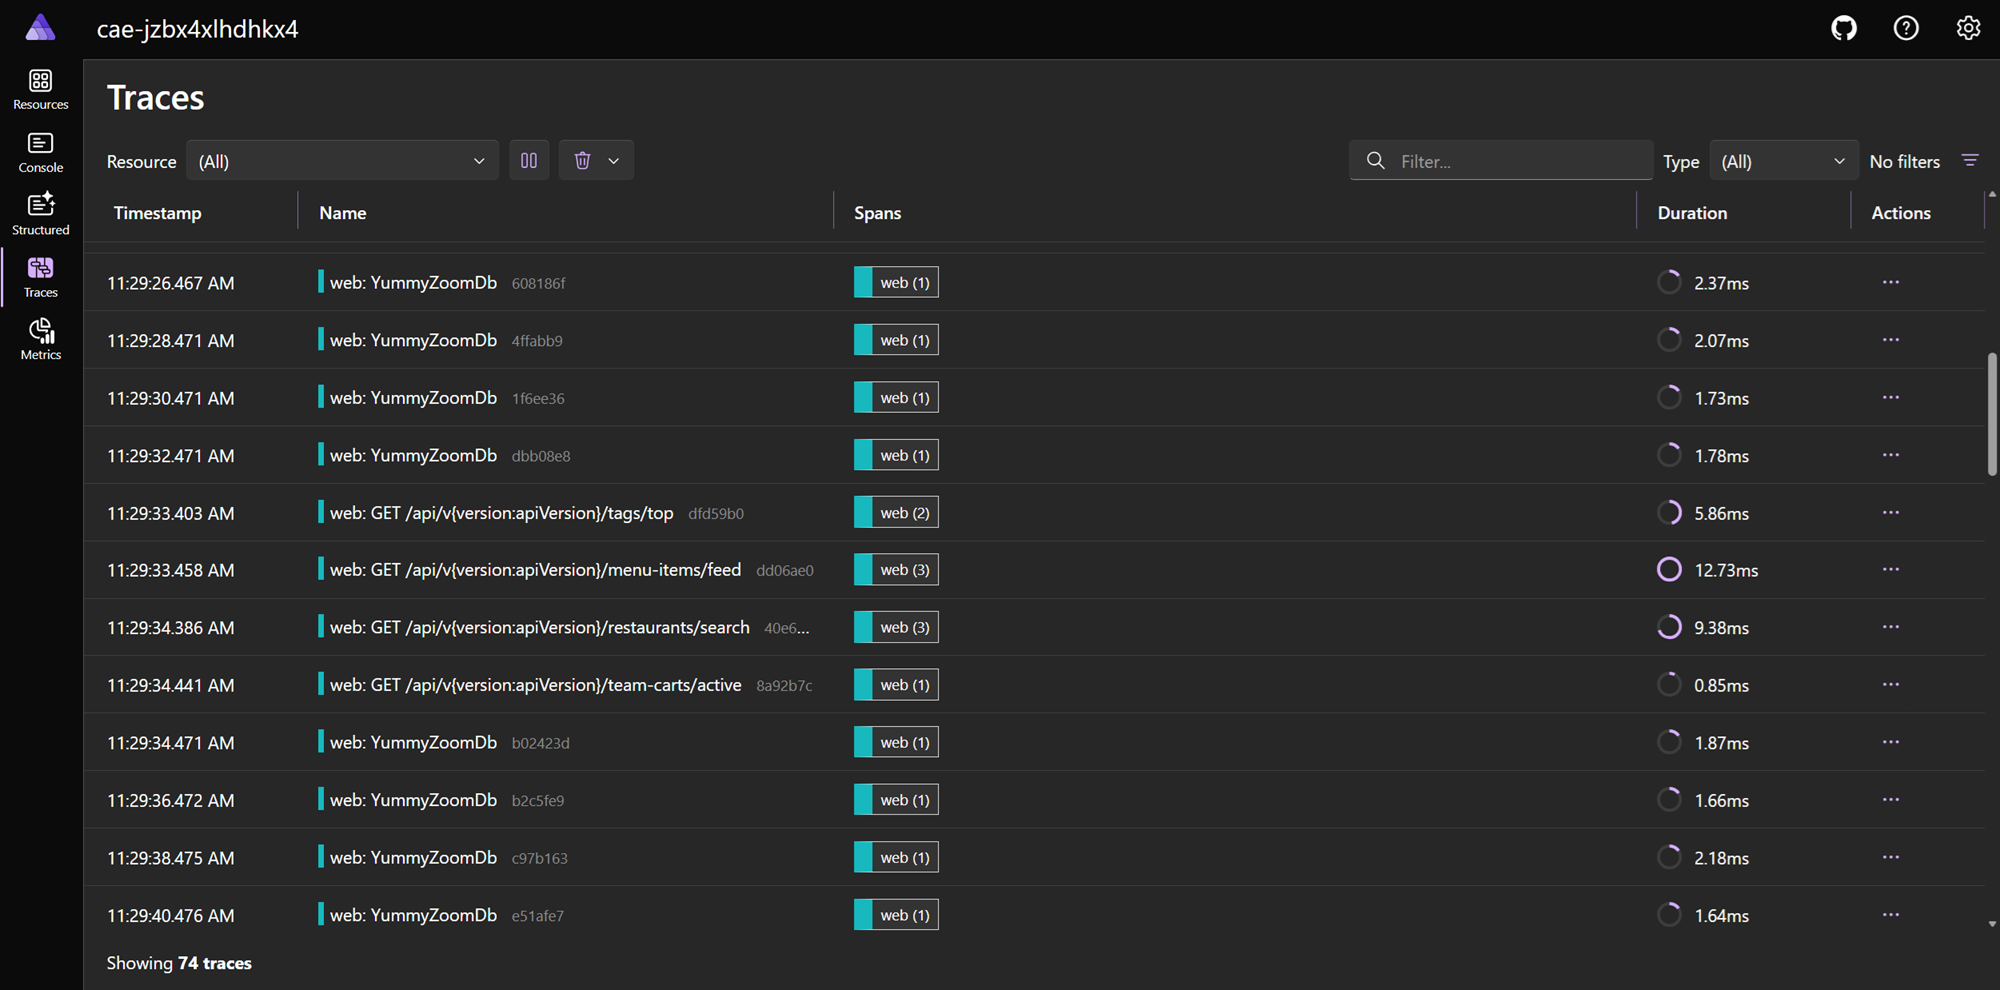
\includegraphics[width=0.95\linewidth]{Dashboard-Traces}
    \caption{Danh sách các Trace thu thập được từ Web API}
    \label{fig:dashboard-traces}
\end{figure}

\begin{figure}[H]
    \centering
    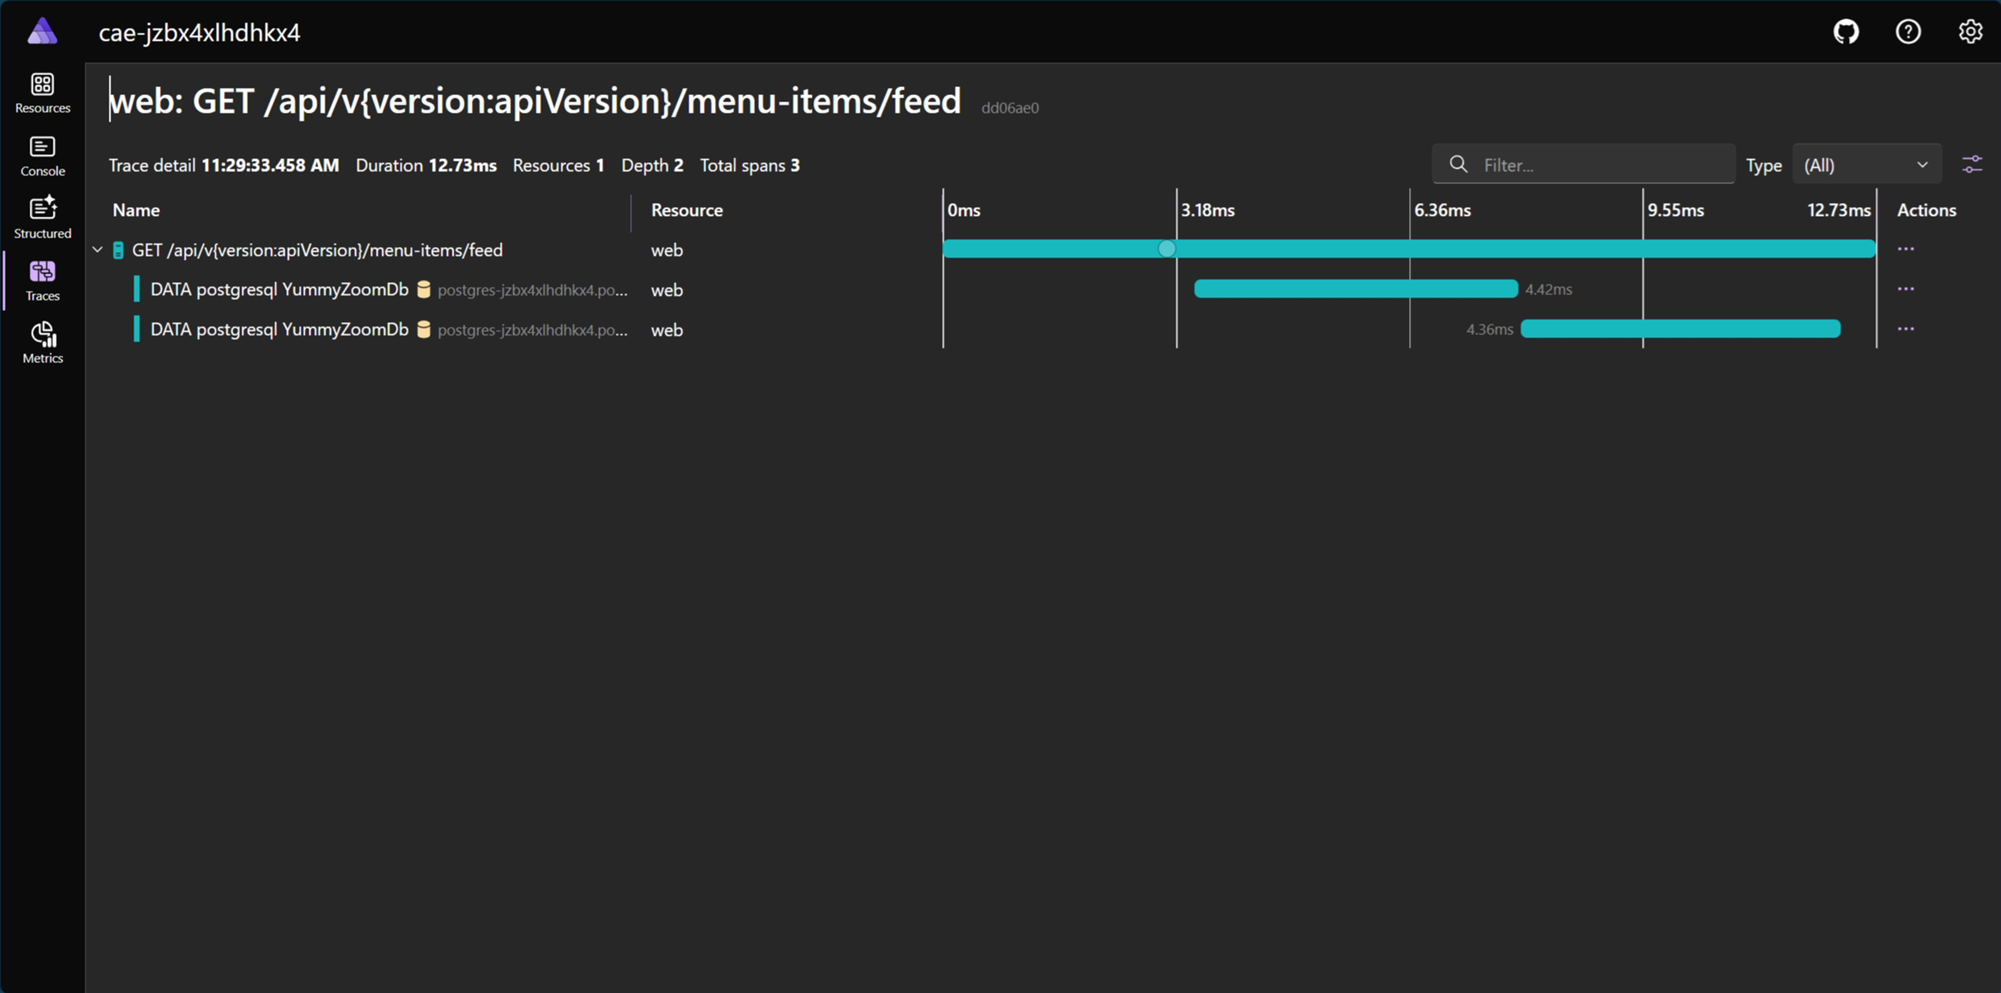
\includegraphics[width=0.95\linewidth]{Dashboard-Traces-Detail}
    \caption{Chi tiết Timeline của một Trace: Phân tích thời gian xử lý từng bước}
    \label{fig:dashboard-traces-detail}
\end{figure}

\section{Chiến lược Mở rộng (Scaling) và Tối ưu chi phí}

Đối với một dự án ở giai đoạn MVP (Minimum Viable Product), việc cân đối giữa hiệu năng và chi phí vận hành là ưu tiên hàng đầu. Đồ án sử dụng tính năng KEDA (Kubernetes Event-driven Autoscaling) có sẵn trong Azure Container Apps để tự động hóa việc mở rộng.

\subsection{Cấu hình Scaling}
Hệ thống được cấu hình để tự động mở rộng (Auto-scaling) dựa trên số lượng request HTTP hoặc kết nối TCP đồng thời.
\begin{itemize}
    \item \textbf{Redis}: Sử dụng rule `tcp-scaling` với ngưỡng 10 kết nối đồng thời. Trong chiến lược mở rộng, Redis không chỉ đóng vai trò là bộ nhớ đệm, mà còn là thành phần cốt lõi đóng vai trò Backplane cho SignalR. Khi hệ thống tự động mở rộng ra nhiều bản sao (Replicas), Redis đảm bảo rằng thông báo về trạng thái giỏ hàng nhóm (TeamCart) được đồng bộ tức thời giữa các instance, giúp người dùng luôn nhìn thấy dữ liệu nhất quán bất kể họ đang kết nối tới container nào.
    \item \textbf{Web API}: Sử dụng rule `http-scaling` với ngưỡng 10 requests đồng thời.
\end{itemize}

\subsection{Bài toán Cold Start và Chi phí}
Một quyết định thiết kế quan trọng trong đồ án là thiết lập `minReplicas = 0` cho cả dịch vụ Redis và Web API.
\begin{itemize}
    \item \textbf{Lý do}: Web API có các tác vụ nền (Background Jobs) chạy định kỳ mỗi 5 phút/lần, việc đặt `minReplicas = 1` sẽ khiến container phải chạy liên tục 24/7, dẫn đến phát sinh chi phí ngay cả khi không có người dùng truy cập.
    \item \textbf{Đánh đổi (Trade-off)}: Chấp nhận hiện tượng "Khởi động nguội" (Cold Start) - request đầu tiên sau một khoảng thời gian nghỉ sẽ chậm hơn bình thường (do Azure phải cấp phát lại container). Đây là sự đánh đổi hợp lý và có tính toán về mặt kinh tế cho môi trường Dev/Test và MVP. Để khắc phục điều này khi đưa vào môi trường sản phẩm thực tế, hệ thống sẽ được áp dụng các quy tắc lập lịch (Scaling Schedules), đảm bảo duy trì ít nhất một instance hoạt động (`minReplicas = 1`) trong các khung giờ cao điểm đặt hàng, và chỉ tự động đưa về 0 vào các khung giờ thấp điểm (ví dụ sau 12h đêm) để tiết kiệm ngân sách hạ tầng.
\end{itemize}

\section*{Kết chương}

Chương này đã trình bày cách hệ thống được quan sát và vận hành thông qua các công cụ hiện đại như OpenTelemetry và Aspire Dashboard, cũng như chiến lược scaling "scale-to-zero" để tiết kiệm chi phí. Phần kết luận sau đây sẽ tổng kết lại toàn bộ đồ án và đề xuất hướng phát triển trong tương lai.

% ==================================================

\chapter*{Kết luận}
\addcontentsline{toc}{chapter}{Kết luận}

Báo cáo này đã trình bày toàn diện quy trình xây dựng và triển khai hạ tầng cho hệ thống YummyZoom trên nền tảng Microsoft Azure. Thông qua việc áp dụng các công nghệ tiên tiến như .NET Aspire và Bicep, đồ án đã giải quyết thành công bài toán về sự phức tạp trong vận hành microservices.

Dự án đã đạt được những kết quả quan trọng trong việc hiện đại hóa quy trình phát triển. Cụ thể, toàn bộ hạ tầng đã được chuyển đổi sang dạng mã nguồn (IaC), đảm bảo tính nhất quán và khả năng kiểm soát phiên bản chặt chẽ giữa các môi trường. Bên cạnh đó, việc xây dựng thành công pipeline CI/CD tự động hóa đã loại bỏ các rủi ro từ thao tác thủ công và rút ngắn đáng kể thời gian đưa tính năng mới đến tay người dùng. Về mặt an toàn và giám sát, hệ thống đã loại bỏ hoàn toàn việc lưu trữ mật khẩu tĩnh nhờ cơ chế Managed Identity, đồng thời cung cấp khả năng quan sát thời gian thực thông qua OpenTelemetry và Aspire Dashboard.

Mặc dù hệ thống hiện tại đã đáp ứng tốt các yêu cầu của giai đoạn MVP, vẫn còn nhiều tiềm năng để tối ưu hóa trong tương lai. Hướng phát triển tiếp theo sẽ tập trung vào việc tinh chỉnh chi phí vận hành thông qua các quy tắc Scaling chi tiết hơn và tận dụng tài nguyên Azure Spot. Ngoài ra, tính sẵn sàng cao (High Availability) cũng sẽ được nâng cấp bằng cách triển khai cơ sở dữ liệu đa vùng (Zone Redundancy), song song với việc tăng cường bảo mật lớp ứng dụng bằng Web Application Firewall (WAF) để chống lại các mối đe dọa mạng ngày càng phức tạp.

Việc hoàn thiện hạ tầng này là tiền đề vững chắc để YummyZoom có thể mở rộng quy mô phục vụ hàng ngàn người dùng trong tương lai.

\end{document}
